\documentclass[
  shownotes,
  xcolor={svgnames},
  hyperref={colorlinks,citecolor=DarkBlue,linkcolor=DarkRed,urlcolor=DarkBlue}
  ]{beamer}
\usepackage{animate}
\usepackage{amsmath}
\usepackage{amsfonts}
\usepackage{amssymb}
\usepackage{pifont}
\usepackage{mathpazo}
%\usepackage{xcolor}
\usepackage{multimedia}
\usepackage{fancybox}
\usepackage[para]{threeparttable}
\usepackage{multirow}
\setcounter{MaxMatrixCols}{30}
\usepackage{subcaption}
\usepackage{graphicx}
\usepackage{lscape}
\usepackage[compatibility=false,font=small]{caption}
\usepackage{booktabs}
\usepackage{ragged2e}
\usepackage{chronosys}
\usepackage{appendixnumberbeamer}
\usepackage{animate}
\setbeamertemplate{caption}[numbered]
\usepackage{color}
%\usepackage{times}
\usepackage{tikz}
\usepackage{comment} %to comment
%% BibTeX settings
\usepackage{natbib}
\bibliographystyle{apalike}
\bibpunct{(}{)}{,}{a}{,}{,}
\setbeamertemplate{bibliography item}{[\theenumiv]}

% Defines columns for bespoke tables
\usepackage{array}
\newcolumntype{L}[1]{>{\raggedright\let\newline\\\arraybackslash\hspace{0pt}}m{#1}}
\newcolumntype{C}[1]{>{\centering\let\newline\\\arraybackslash\hspace{0pt}}m{#1}}
\newcolumntype{R}[1]{>{\raggedleft\let\newline\\\arraybackslash\hspace{0pt}}m{#1}}


\usepackage{xfrac}


\usepackage{multicol}
\setlength{\columnsep}{0.5cm}

% Theme and colors
\usetheme{Boadilla}

% I use steel blue and a custom color palette. This defines it.
\definecolor{andesred}{HTML}{af2433}

% Other options
\providecommand{\U}[1]{\protect\rule{.1in}{.1in}}
\usefonttheme{serif}
\setbeamertemplate{itemize items}[default]
\setbeamertemplate{enumerate items}[square]
\setbeamertemplate{section in toc}[circle]

\makeatletter

\definecolor{mybackground}{HTML}{82CAFA}
\definecolor{myforeground}{HTML}{0000A0}

\setbeamercolor{normal text}{fg=black,bg=white}
\setbeamercolor{alerted text}{fg=red}
\setbeamercolor{example text}{fg=black}

\setbeamercolor{background canvas}{fg=myforeground, bg=white}
\setbeamercolor{background}{fg=myforeground, bg=mybackground}

\setbeamercolor{palette primary}{fg=black, bg=gray!30!white}
\setbeamercolor{palette secondary}{fg=black, bg=gray!20!white}
\setbeamercolor{palette tertiary}{fg=white, bg=andesred}

\setbeamercolor{frametitle}{fg=andesred}
\setbeamercolor{title}{fg=andesred}
\setbeamercolor{block title}{fg=andesred}
\setbeamercolor{itemize item}{fg=andesred}
\setbeamercolor{itemize subitem}{fg=andesred}
\setbeamercolor{itemize subsubitem}{fg=andesred}
\setbeamercolor{enumerate item}{fg=andesred}
\setbeamercolor{item projected}{bg=gray!30!white,fg=andesred}
\setbeamercolor{enumerate subitem}{fg=andesred}
\setbeamercolor{section number projected}{bg=gray!30!white,fg=andesred}
\setbeamercolor{section in toc}{fg=andesred}
\setbeamercolor{caption name}{fg=andesred}
\setbeamercolor{button}{bg=gray!30!white,fg=andesred}


\usepackage{fancyvrb}
\newcommand{\VerbBar}{|}
\newcommand{\VERB}{\Verb[commandchars=\\\{\}]}
\DefineVerbatimEnvironment{Highlighting}{Verbatim}{commandchars=\\\{\}}
% Add ',fontsize=\small' for more characters per line
\usepackage{framed}
\definecolor{shadecolor}{RGB}{248,248,248}
\newenvironment{Shaded}{\begin{snugshade}}{\end{snugshade}}
\newcommand{\AlertTok}[1]{\textcolor[rgb]{0.94,0.16,0.16}{#1}}
\newcommand{\AnnotationTok}[1]{\textcolor[rgb]{0.56,0.35,0.01}{\textbf{\textit{#1}}}}
\newcommand{\AttributeTok}[1]{\textcolor[rgb]{0.77,0.63,0.00}{#1}}
\newcommand{\BaseNTok}[1]{\textcolor[rgb]{0.00,0.00,0.81}{#1}}
\newcommand{\BuiltInTok}[1]{#1}
\newcommand{\CharTok}[1]{\textcolor[rgb]{0.31,0.60,0.02}{#1}}
\newcommand{\CommentTok}[1]{\textcolor[rgb]{0.56,0.35,0.01}{\textit{#1}}}
\newcommand{\CommentVarTok}[1]{\textcolor[rgb]{0.56,0.35,0.01}{\textbf{\textit{#1}}}}
\newcommand{\ConstantTok}[1]{\textcolor[rgb]{0.00,0.00,0.00}{#1}}
\newcommand{\ControlFlowTok}[1]{\textcolor[rgb]{0.13,0.29,0.53}{\textbf{#1}}}
\newcommand{\DataTypeTok}[1]{\textcolor[rgb]{0.13,0.29,0.53}{#1}}
\newcommand{\DecValTok}[1]{\textcolor[rgb]{0.00,0.00,0.81}{#1}}
\newcommand{\DocumentationTok}[1]{\textcolor[rgb]{0.56,0.35,0.01}{\textbf{\textit{#1}}}}
\newcommand{\ErrorTok}[1]{\textcolor[rgb]{0.64,0.00,0.00}{\textbf{#1}}}
\newcommand{\ExtensionTok}[1]{#1}
\newcommand{\FloatTok}[1]{\textcolor[rgb]{0.00,0.00,0.81}{#1}}
\newcommand{\FunctionTok}[1]{\textcolor[rgb]{0.00,0.00,0.00}{#1}}
\newcommand{\ImportTok}[1]{#1}
\newcommand{\InformationTok}[1]{\textcolor[rgb]{0.56,0.35,0.01}{\textbf{\textit{#1}}}}
\newcommand{\KeywordTok}[1]{\textcolor[rgb]{0.13,0.29,0.53}{\textbf{#1}}}
\newcommand{\NormalTok}[1]{#1}
\newcommand{\OperatorTok}[1]{\textcolor[rgb]{0.81,0.36,0.00}{\textbf{#1}}}
\newcommand{\OtherTok}[1]{\textcolor[rgb]{0.56,0.35,0.01}{#1}}
\newcommand{\PreprocessorTok}[1]{\textcolor[rgb]{0.56,0.35,0.01}{\textit{#1}}}
\newcommand{\RegionMarkerTok}[1]{#1}
\newcommand{\SpecialCharTok}[1]{\textcolor[rgb]{0.00,0.00,0.00}{#1}}
\newcommand{\SpecialStringTok}[1]{\textcolor[rgb]{0.31,0.60,0.02}{#1}}
\newcommand{\StringTok}[1]{\textcolor[rgb]{0.31,0.60,0.02}{#1}}
\newcommand{\VariableTok}[1]{\textcolor[rgb]{0.00,0.00,0.00}{#1}}
\newcommand{\VerbatimStringTok}[1]{\textcolor[rgb]{0.31,0.60,0.02}{#1}}
\newcommand{\WarningTok}[1]{\textcolor[rgb]{0.56,0.35,0.01}{\textbf{\textit{#1}}}}
\usepackage{graphicx}
\makeatletter

\usepackage{tikz}
% Tikz settings optimized for causal graphs.
\usetikzlibrary{shapes,decorations,arrows,calc,arrows.meta,fit,positioning}
\tikzset{
    -Latex,auto,node distance =1 cm and 1 cm,semithick,
    state/.style ={ellipse, draw, minimum width = 0.7 cm},
    point/.style = {circle, draw, inner sep=0.04cm,fill,node contents={}},
    bidirected/.style={Latex-Latex,dashed},
    el/.style = {inner sep=2pt, align=left, sloped}
}


\makeatother






%%%%%%%%%%%%%%% BEGINS DOCUMENT %%%%%%%%%%%%%%%%%%

\begin{document}

\title[Lecture 12]{Lecture 12: \\ Spatial Dependence}
\subtitle{Big Data and Machine Learning for Applied Economics \\ Econ 4676}
\date{\today}

\author[Sarmiento-Barbieri]{Ignacio Sarmiento-Barbieri}
\institute[Uniandes]{Universidad de los Andes}


\begin{frame}[noframenumbering]
\maketitle
\end{frame}

%%%%%%%%%%%%%%%%%%%%%%%%%%%%%%%%%%%


%----------------------------------------------------------------------%
\begin{frame}
\frametitle{Recap }

  \begin{itemize} 
      \item Types of Spatial Data
      \medskip
      \item Reading and Mapping spatial data in R
      \medskip
      \item Projections
      \medskip
      \item Creating Spatial Objects
      \medskip
      \item Measuring Distances
  \end{itemize}

\end{frame}

%----------------------------------------------------------------------% 

\begin{frame}
\frametitle{Agenda}

\tableofcontents

\end{frame}




%----------------------------------------------------------------------%
\section{Motivation }
%----------------------------------------------------------------------%
\begin{frame}[fragile]
\frametitle{Motivation}


\begin{minipage}[t]{0.52\linewidth}
\bigskip
\begin{itemize}
  
  \item Independence assumption between observation is no longer valid
  \medskip
  \item Attributes of observation $i$  may influence the attributes of observation $j$.
  \medskip
  \item We will consider various alternatives to model spatial dependence
  \medskip
  \item Think as a way to model $f(X)$
\end{itemize}

    \end{minipage}
    \hfill
    \begin{minipage}[t]{0.43\linewidth}%
       \medskip
        \begin{figure}[H] \centering
            \captionsetup{justification=centering}
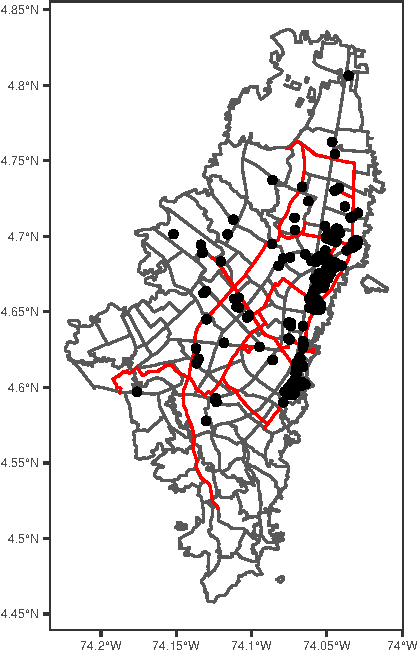
\includegraphics[scale=0.6]{figures/restaurants_bogota.pdf}

 \end{figure}
    \end{minipage}

\end{frame}

%----------------------------------------------------------------------%
\begin{frame}[fragile]
\frametitle{Motivation}


    \begin{minipage}[t]{0.52\linewidth}
\bigskip
\begin{itemize}
  \small
  \item Independence assumption between observation is no longer valid
  \medskip
  \item Attributes of observation $i$  may influence the attributes of observation $j$.
  \medskip
  \item Positive Spatial correlation arises when units that are {\it close} to one another are more similar than units that are far apart
  \medskip
  \item Similarly spatial heterogeneity arises when some areas present more variability than others
\end{itemize}

    \end{minipage}
    \hfill
    \begin{minipage}[t]{0.43\linewidth}%
       \medskip
        \begin{figure}[H] 
          \begin{subfigure}{0.45\linewidth}
          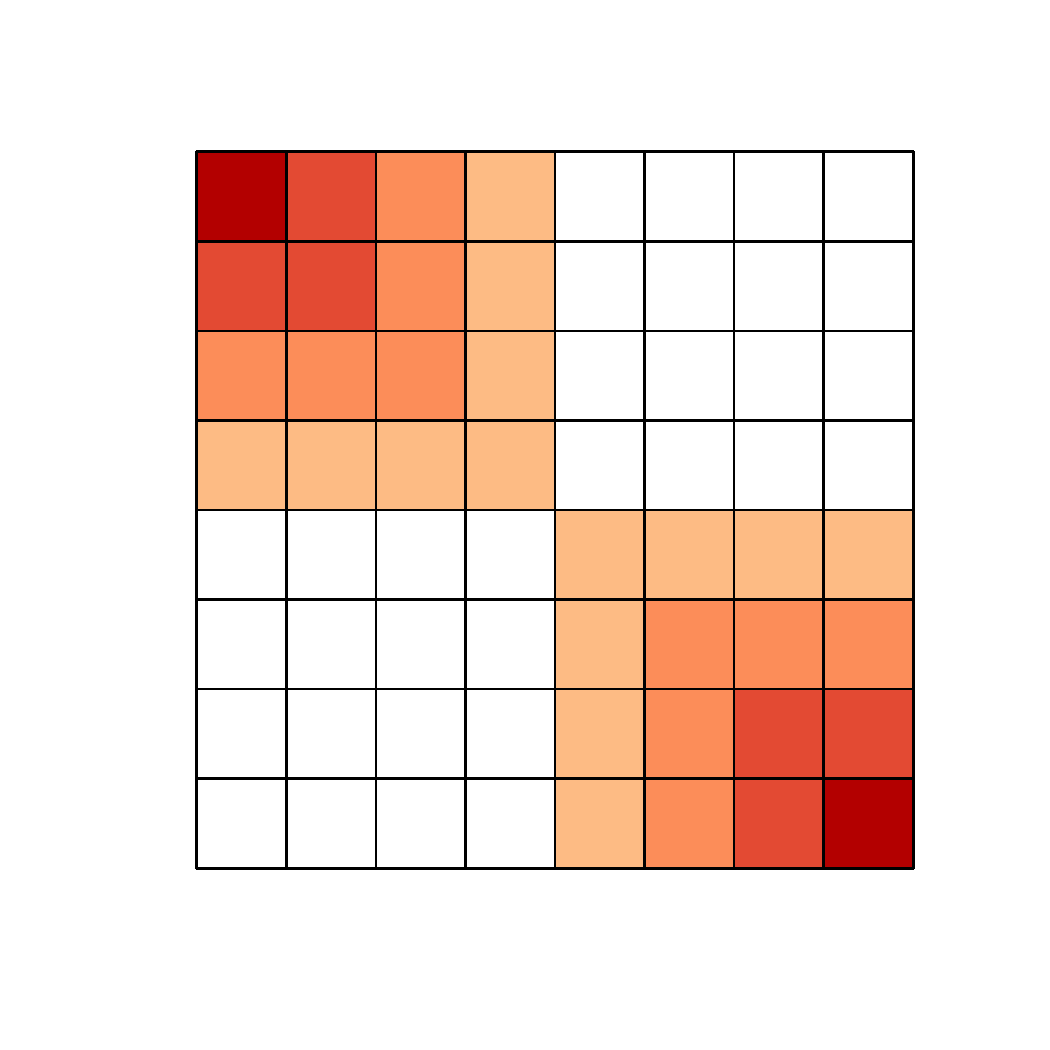
\includegraphics[scale=.21]{figures/spatial_correlation.pdf}
          \end{subfigure} \\
          
          \begin{subfigure}{0.45\linewidth}
          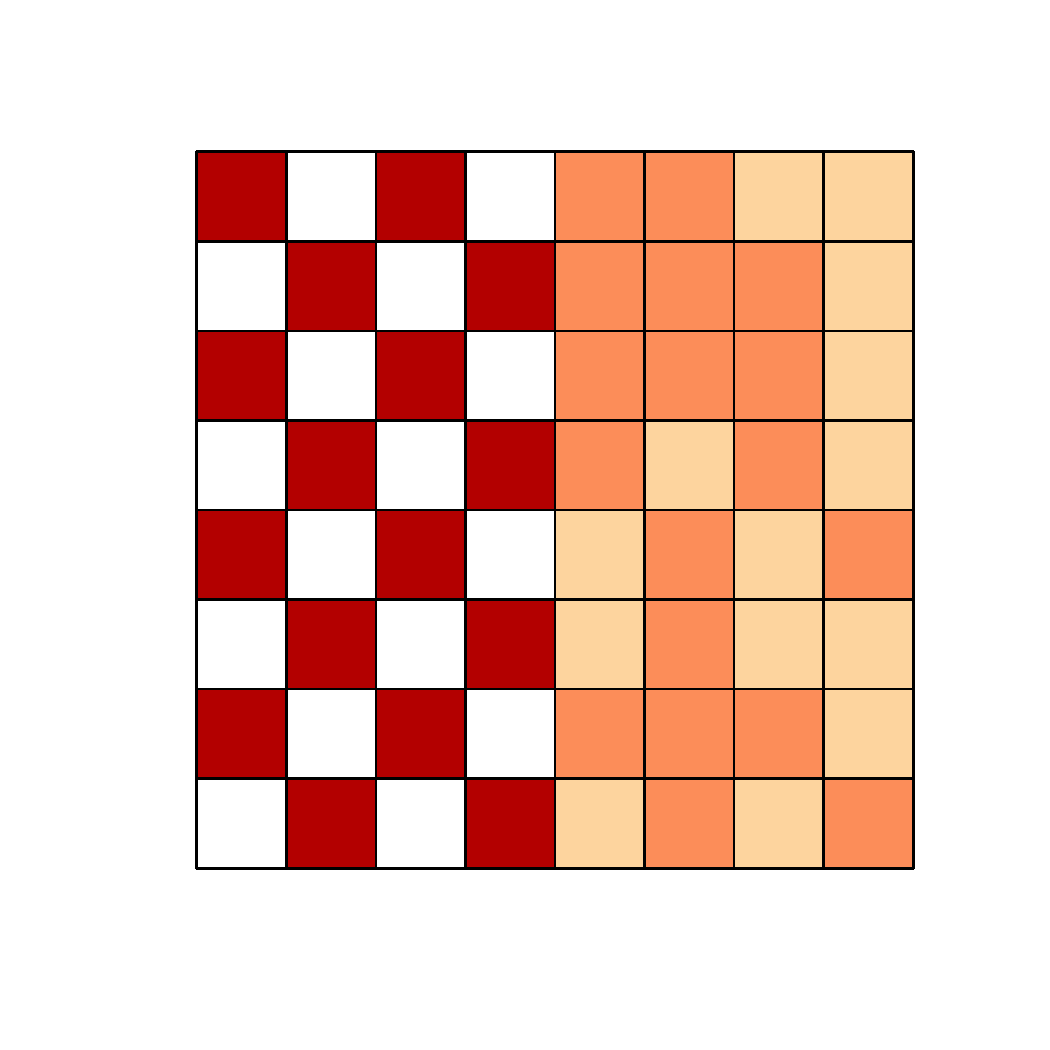
\includegraphics[scale=.21]{figures/spatial_heterogeneity.pdf}
          \end{subfigure}

  \end{figure}
    \end{minipage}

\end{frame}
%----------------------------------------------------------------------%
\section{Closeness }
%----------------------------------------------------------------------%
\begin{frame}[fragile]
\frametitle{Closeness}

 {\it “Everything is related to everything else, but close things are more related than things that are far apart”} (Tobler, 1979).

\bigskip

\begin{itemize}
  \item One of the major differences between standard econometrics and standard spatial econometrics lies, in the fact that, in order to treat spatial data, we need to use two different sets of information
  \medskip
  \begin{enumerate}
  \item Observed values of the economic variables
  \medskip
  \item Particular location where those variables are observed and to the various links of proximity between all spatial observations
  \end{enumerate}
\end{itemize}

\end{frame}
%----------------------------------------------------------------------%
\begin{frame}[fragile]
\frametitle{Closeness}

\bigskip

\begin{minipage}[t]{0.45\linewidth}
Rook criterion: two units are close to one another if they share a side
  \begin{figure}[H] \centering
    \captionsetup{justification=centering}
    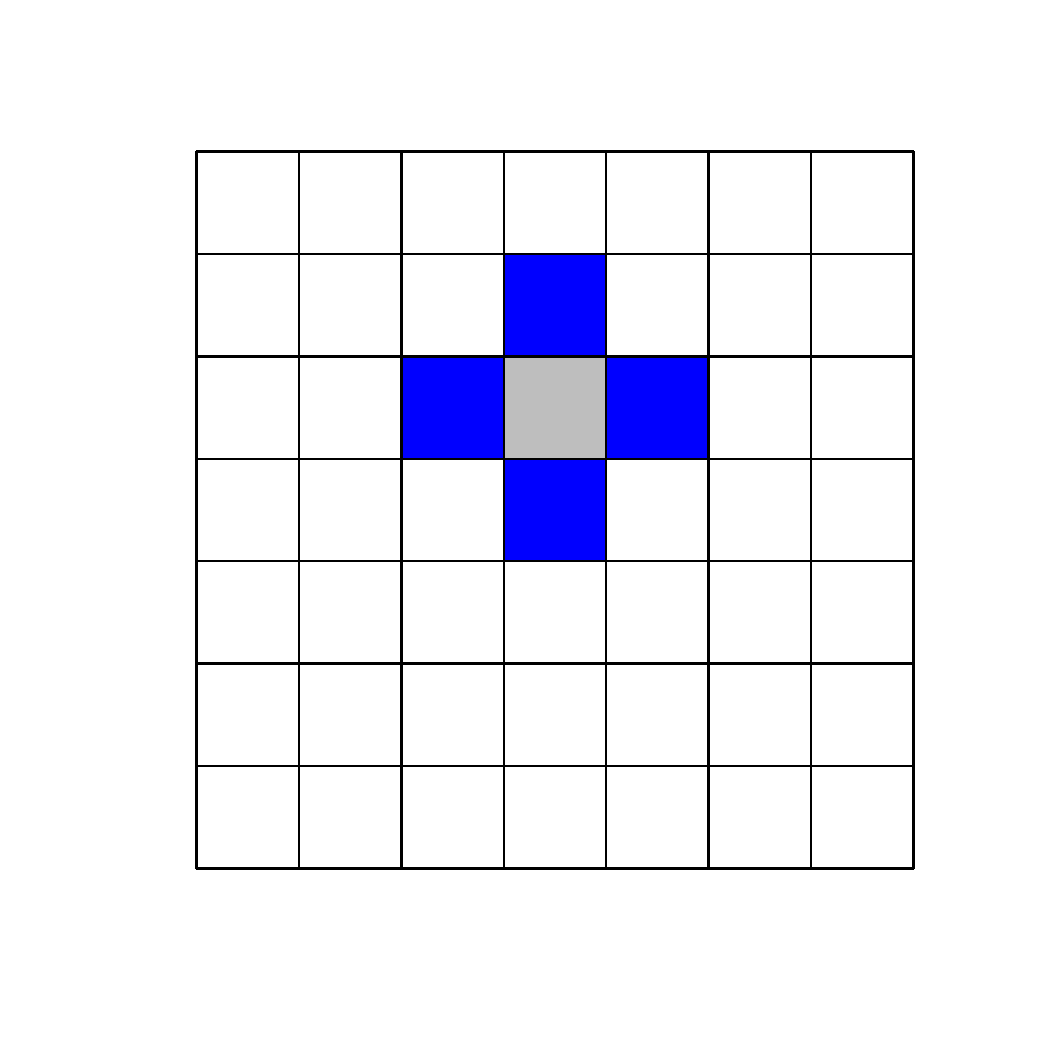
\includegraphics[scale=0.3]{figures/rook.pdf}
   \end{figure}
  
    \end{minipage}
    \hfill
\begin{minipage}[t]{0.45\linewidth}%
Queen criterion: two units are close if they share a side or an edge.
  \begin{figure}[H] \centering
    \captionsetup{justification=centering}
    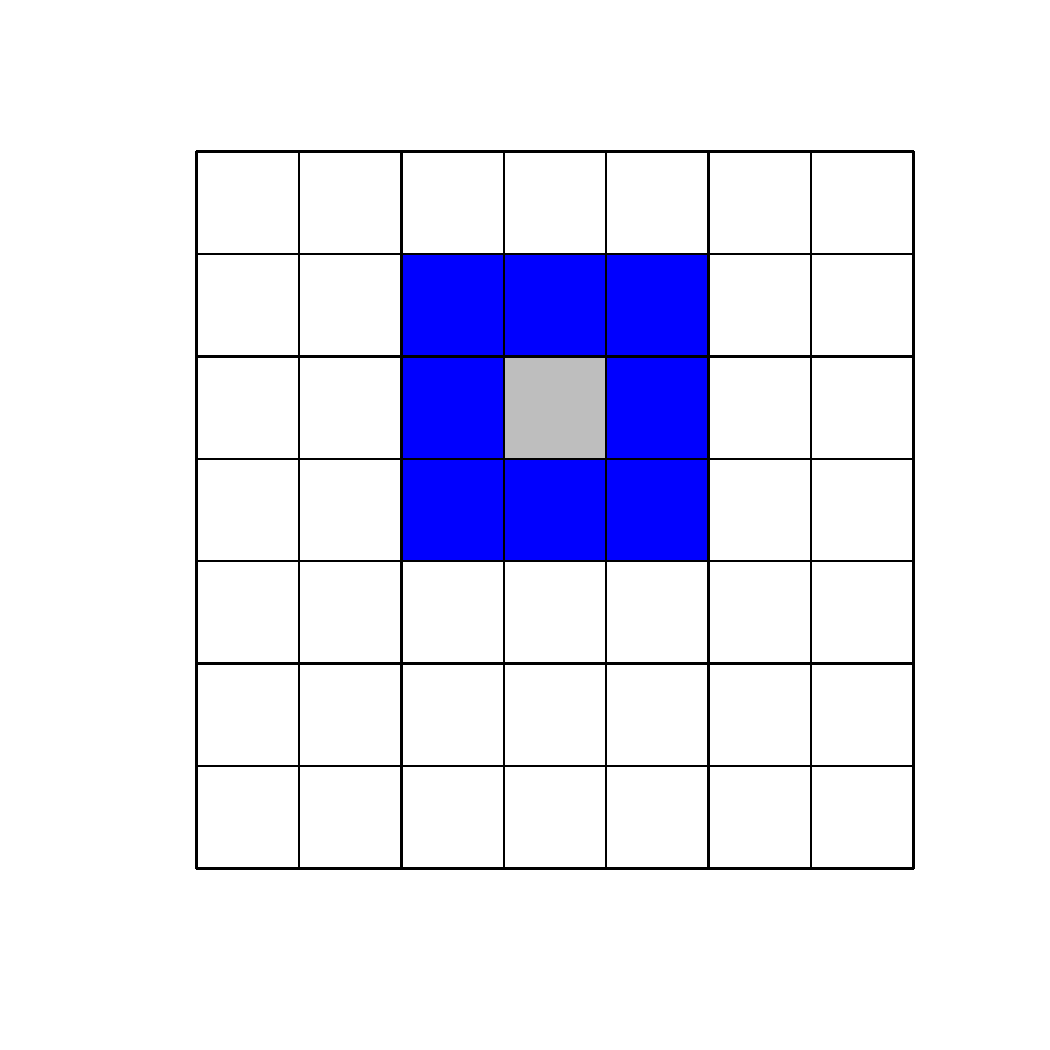
\includegraphics[scale=0.3]{figures/queen.pdf}
   \end{figure}
\end{minipage}


\end{frame}

%----------------------------------------------------------------------%
\section{Weights Matrix}
%----------------------------------------------------------------------%
\begin{frame}[fragile]
\frametitle{Weights Matrix}

\begin{itemize}
  \item At the heart of traditional spatial econometrics is the definition of the {\it weights matrix}:
\end{itemize}


\begin{align}
W=\left(\begin{array}{cccc}
w_{11} & \dots & \dots & w_{n1}\\
\vdots & w_{ij} &  & \vdots\\
\vdots &  & \ddots & \vdots\\
w_{n_{1}} & \dots & \dots & w_{nn}
\end{array}\right)_{n\times n}
\end{align}

with generic element:

\begin{equation}
w_{ij}=\begin{cases}
1 & if\,j\in N\left(i\right)\\
0 & o.w
\end{cases}
\end{equation}

$N(i)$ being the set of neighbors of location $j$. By convention, the diagonal elements are set to zero, i.e. $w_{ii}=0$. 

\end{frame}
%----------------------------------------------------------------------%
\begin{frame}[fragile]
\frametitle{Weights Matrix}



\begin{itemize}
\item The specification of  the neighboring set ($N(i)$) is quite arbitrary and there's a wide range of suggestions in the literature. 
\bigskip
  \begin{itemize}
    \item Rook criterion
    \medskip
    \item Queen criterion
    \medskip
    \item Two observations are neighbors if they are within a certain distance, i.e., $j\in N(j)$ if $d_{ij} < d_{max}$ where $d$ is the distance between location $i$ and $j$. 
    \medskip
    \item Closest neighbor, ties can be solved randomly
    \medskip
    \item More general matrices can also be specified by considering entries of $w_{ij}$ as functions of geographical, economic or social distances between areas rather than simply characterized by dichotomous entries 
  \end{itemize}
\end{itemize}


\end{frame}

%----------------------------------------------------------------------%
\subsection{Examples of Weight Matrices}
%----------------------------------------------------------------------%
\begin{frame}[fragile]
\frametitle{Some Examples of Weights Matrices}


\begin{minipage}[t]{0.53\linewidth}
  \begin{figure}[H] \centering
    \captionsetup{justification=centering}
    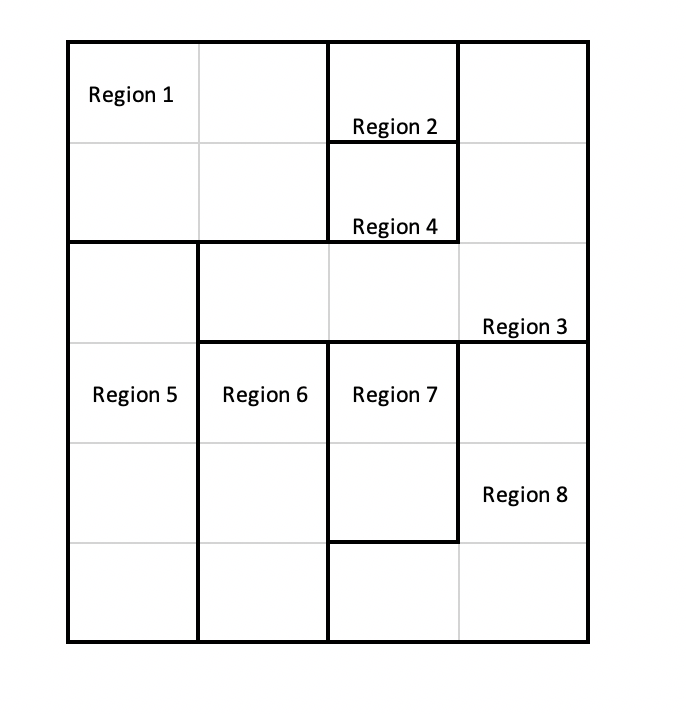
\includegraphics[scale=0.6]{figures/regions_example}
   \end{figure}
  
    \end{minipage}
    \hfill
\begin{minipage}[t]{0.43\linewidth}%
\scriptsize
Adjacency Criterion
\begin{align}
W=\left(\begin{array}{cccccccc}
0 & 1 & 1 & 1 & 1 & 0 & 0 & 0\\
1 & 0 & 1 & 1 & 0 & 0 & 0 & 0\\
1 & 1 & 0 & 1 & 1 & 1 & 1 & 1\\
1 & 1 & 1 & 0 & 0 & 0 & 0 & 0\\
1 & 0 & 1 & 0 & 0 & 1 & 0 & 0\\
0 & 0 & 1 & 0 & 1 & 0 & 1 & 1\\
0 & 0 & 1 & 0 & 0 & 1 & 0 & 1\\
0 & 0 & 1 & 0 & 0 & 1 & 1 & 0
\end{array}\right)_{8\times8} \nonumber
\end{align}
\end{minipage}

\end{frame}
%----------------------------------------------------------------------%
\begin{frame}[fragile]
\frametitle{Some Examples of Weights Matrices}


\begin{minipage}[t]{0.53\linewidth}
  \begin{figure}[H] \centering
    \captionsetup{justification=centering}
    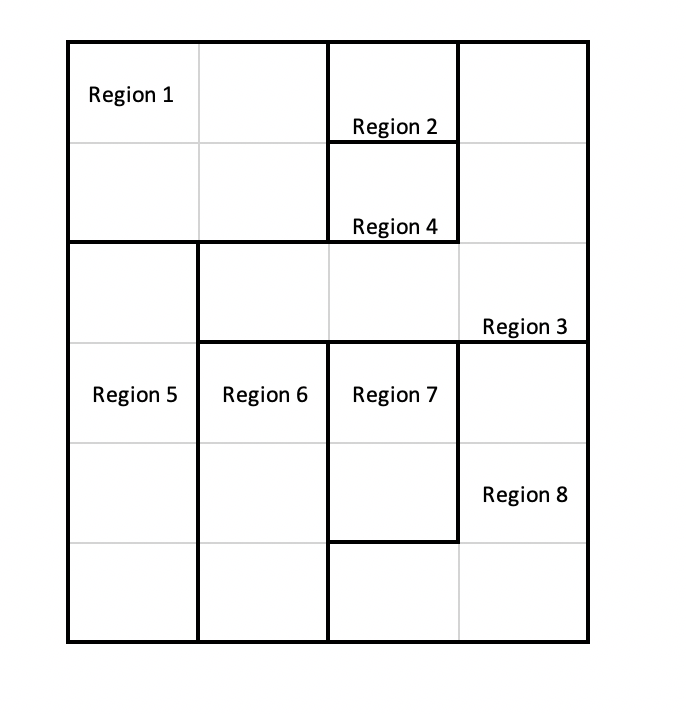
\includegraphics[scale=0.6]{figures/regions_example}
   \end{figure}
  
    \end{minipage}
    \hfill
\begin{minipage}[t]{0.43\linewidth}%
\scriptsize
Nearest Neighbor
\begin{align}
W=\left(\begin{array}{cccccccc}
0 & 1 & 0 & 0 & 0 & 0 & 0 & 0\\
0 & 0 & 0 & 1 & 0 & 0 & 0 & 0\\
0 & 0 & 0 & 1 & 0 & 0 & 0 & 0\\
0 & 1 & 0 & 0 & 0 & 0 & 0 & 0\\
0 & 0 & 0 & 0 & 0 & 1 & 0 & 0\\
0 & 0 & 0 & 0 & 0 & 0 & 1 & 0\\
0 & 0 & 0 & 0 & 0 & 1 & 0 & 0\\
0 & 0 & 0 & 0 & 0 & 0 & 1 & 0
\end{array}\right)_{8\times8} \nonumber
\end{align}
\end{minipage}


\end{frame}
%----------------------------------------------------------------------%
\begin{frame}[fragile]
\frametitle{Some Examples of Weights Matrices}


\begin{minipage}[t]{0.53\linewidth}
  \begin{figure}[H] \centering
    \captionsetup{justification=centering}
    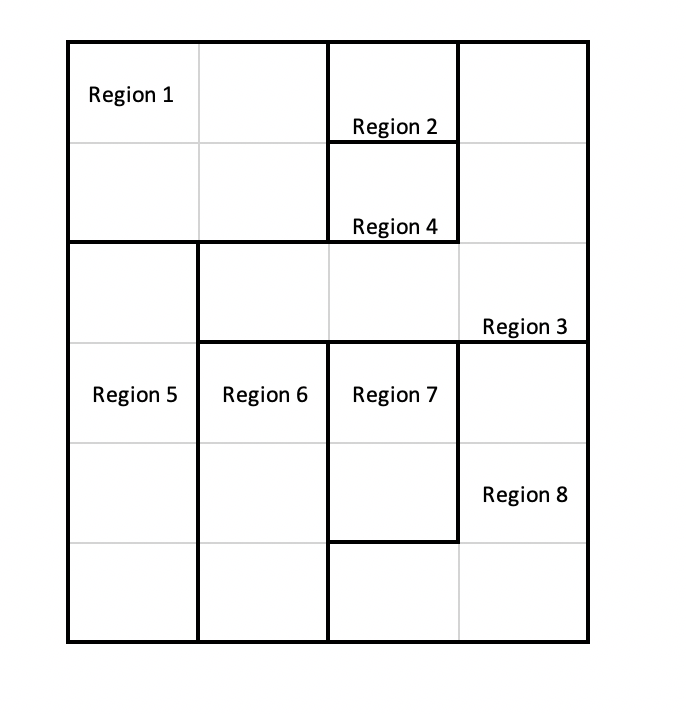
\includegraphics[scale=0.6]{figures/regions_example}
   \end{figure}
  
    \end{minipage}
    \hfill
\begin{minipage}[t]{0.43\linewidth}%
\scriptsize
Distance $<2$
\begin{align}
W=\left(\begin{array}{cccccccc}
0 & 1 & 0 & 1 & 0 & 0 & 0 & 0\\
1 & 0 & 1 & 1 & 0 & 0 & 0 & 0\\
0 & 1 & 0 & 1 & 0 & 0 & 0 & 0\\
1 & 1 & 1 & 0 & 0 & 0 & 0 & 0\\
0 & 0 & 0 & 0 & 0 & 1 & 1 & 0\\
0 & 0 & 0 & 0 & 1 & 0 & 1 & 0\\
0 & 0 & 0 & 0 & 1 & 1 & 0 & 0\\
0 & 0 & 0 & 0 & 0 & 0 & 1 & 0
\end{array}\right)_{8\times8} \nonumber
\end{align}
\end{minipage}

\end{frame}

%----------------------------------------------------------------------%
\begin{frame}[fragile]
\frametitle{Some Examples of Weights Matrices}


  \begin{figure}[H] \centering
    \captionsetup{justification=centering}
    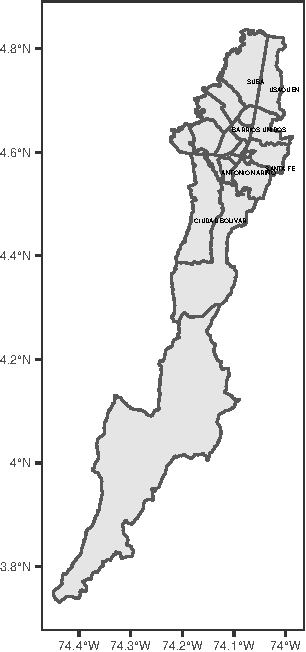
\includegraphics[scale=0.6]{figures/localities.pdf}
   \end{figure}

\end{frame}

%----------------------------------------------------------------------%
\begin{frame}[fragile]
\frametitle{Some Examples of Weights Matrices}

  \begin{figure}[H] \centering
    \captionsetup{justification=centering}
    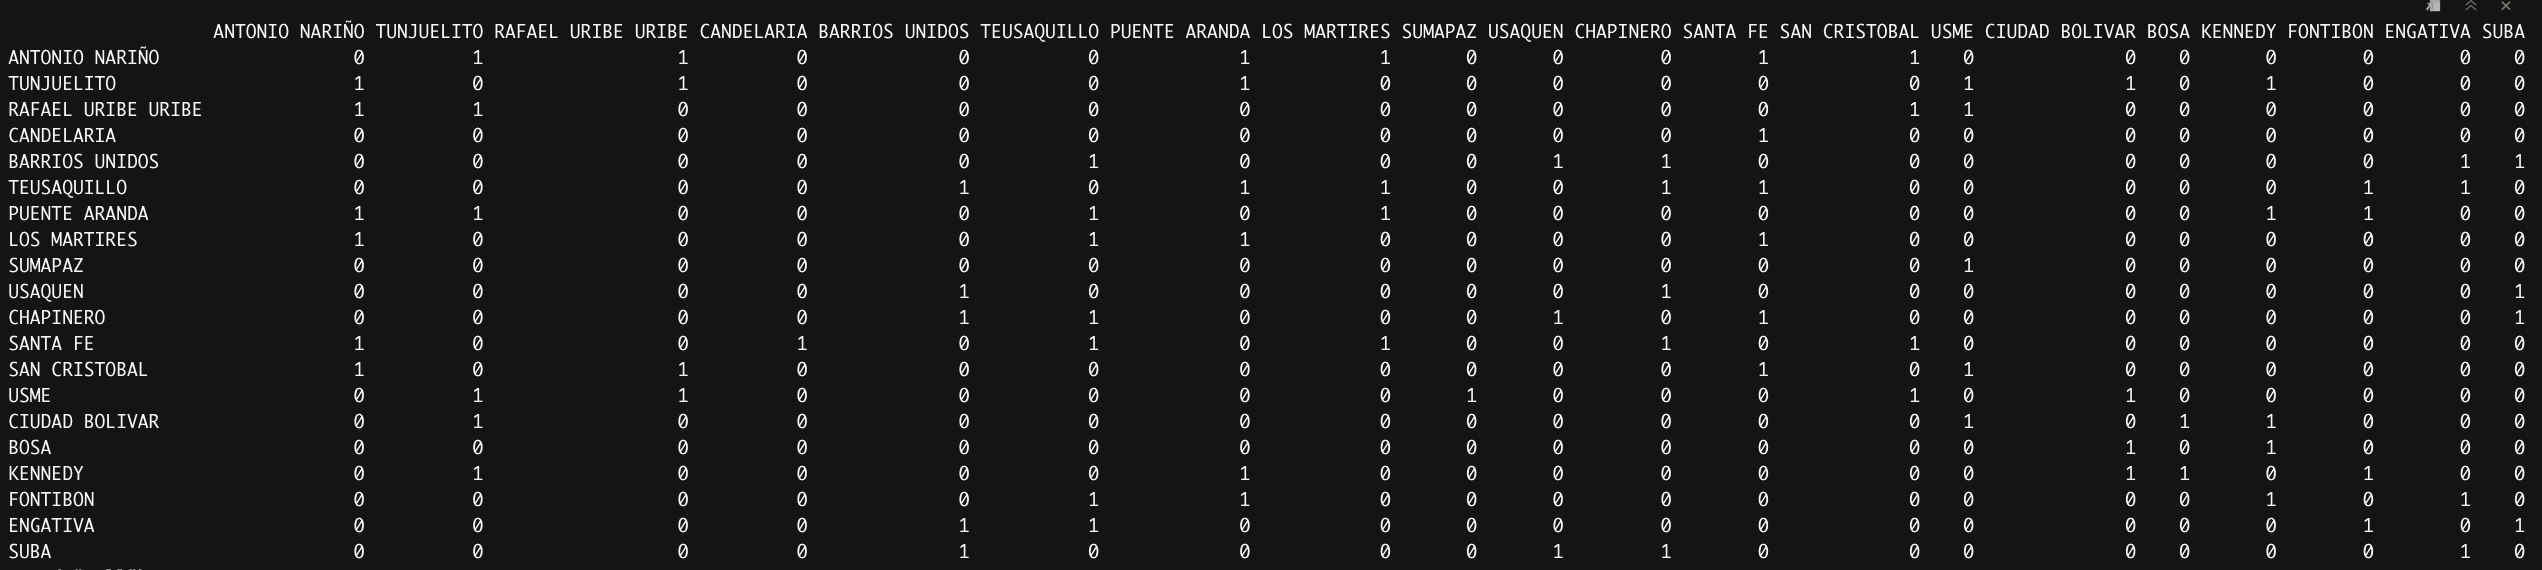
\includegraphics[scale=0.25]{figures/matrix_loc}
   \end{figure}

\end{frame}


%----------------------------------------------------------------------%
\begin{frame}[fragile]
\frametitle{Some Examples of Weights Matrices}
Quite often the $W$ matrices are standardized to sum to one in each row

\begin{align}
w^*_{ij}=\frac{w_{ij}}{\sum_{j=1}^n}w_{ij}
\end{align}

This can be quite useful since

\begin{align}
L(y) =W^{*} y
\end{align}

in which each single element is equal to

\begin{align}
L(y_i) &= \sum_{j=1}^n w^*_{ij}y_j \\ \nonumber
&= \sum_{j=1}^n \frac{w_{ij}y_j}{\sum_{j=1}^n w_{ij}}  \\
&= \frac{\sum_{j\in N(i)}y_j}{\# N(i)}
\end{align}
\end{frame}
%----------------------------------------------------------------------%
\begin{frame}[fragile]
\frametitle{Some Examples of Weights Matrices}

  \begin{figure}[H] \centering
    \captionsetup{justification=centering}
    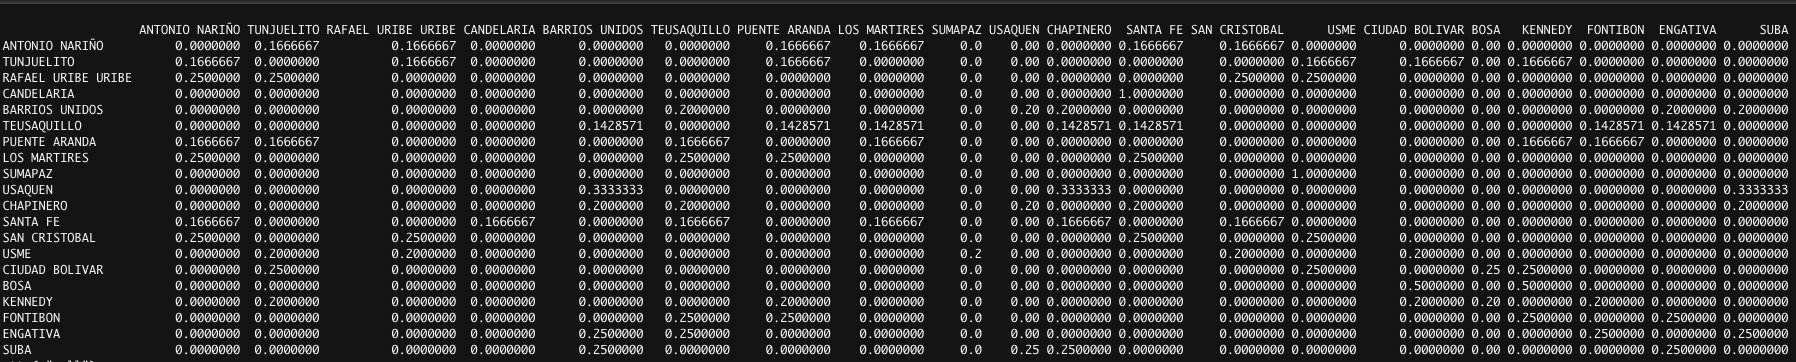
\includegraphics[scale=0.45]{figures/matrix_loc_row_stand}
   \end{figure}

\end{frame}

%----------------------------------------------------------------------%
\begin{frame}[fragile]
\frametitle{Some Examples of Weights Matrices}


  \begin{figure}[H] \centering
    \captionsetup{justification=centering}
    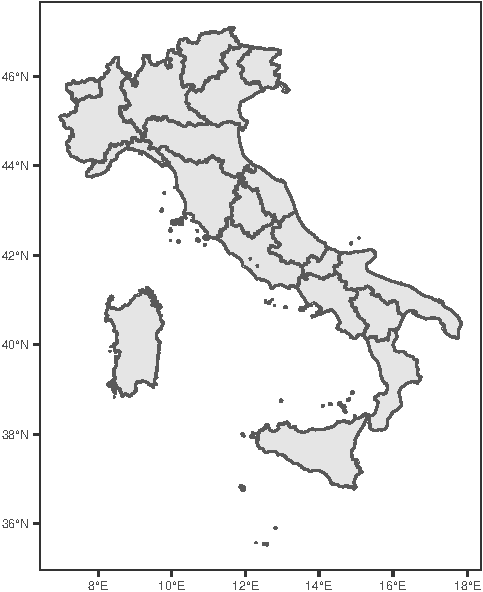
\includegraphics[scale=0.6]{figures/italia.pdf}
   \end{figure}

\end{frame}

%----------------------------------------------------------------------%
\begin{frame}[fragile]
\frametitle{Some Examples of Weights Matrices}


  \begin{figure}[H] \centering
    \captionsetup{justification=centering}
    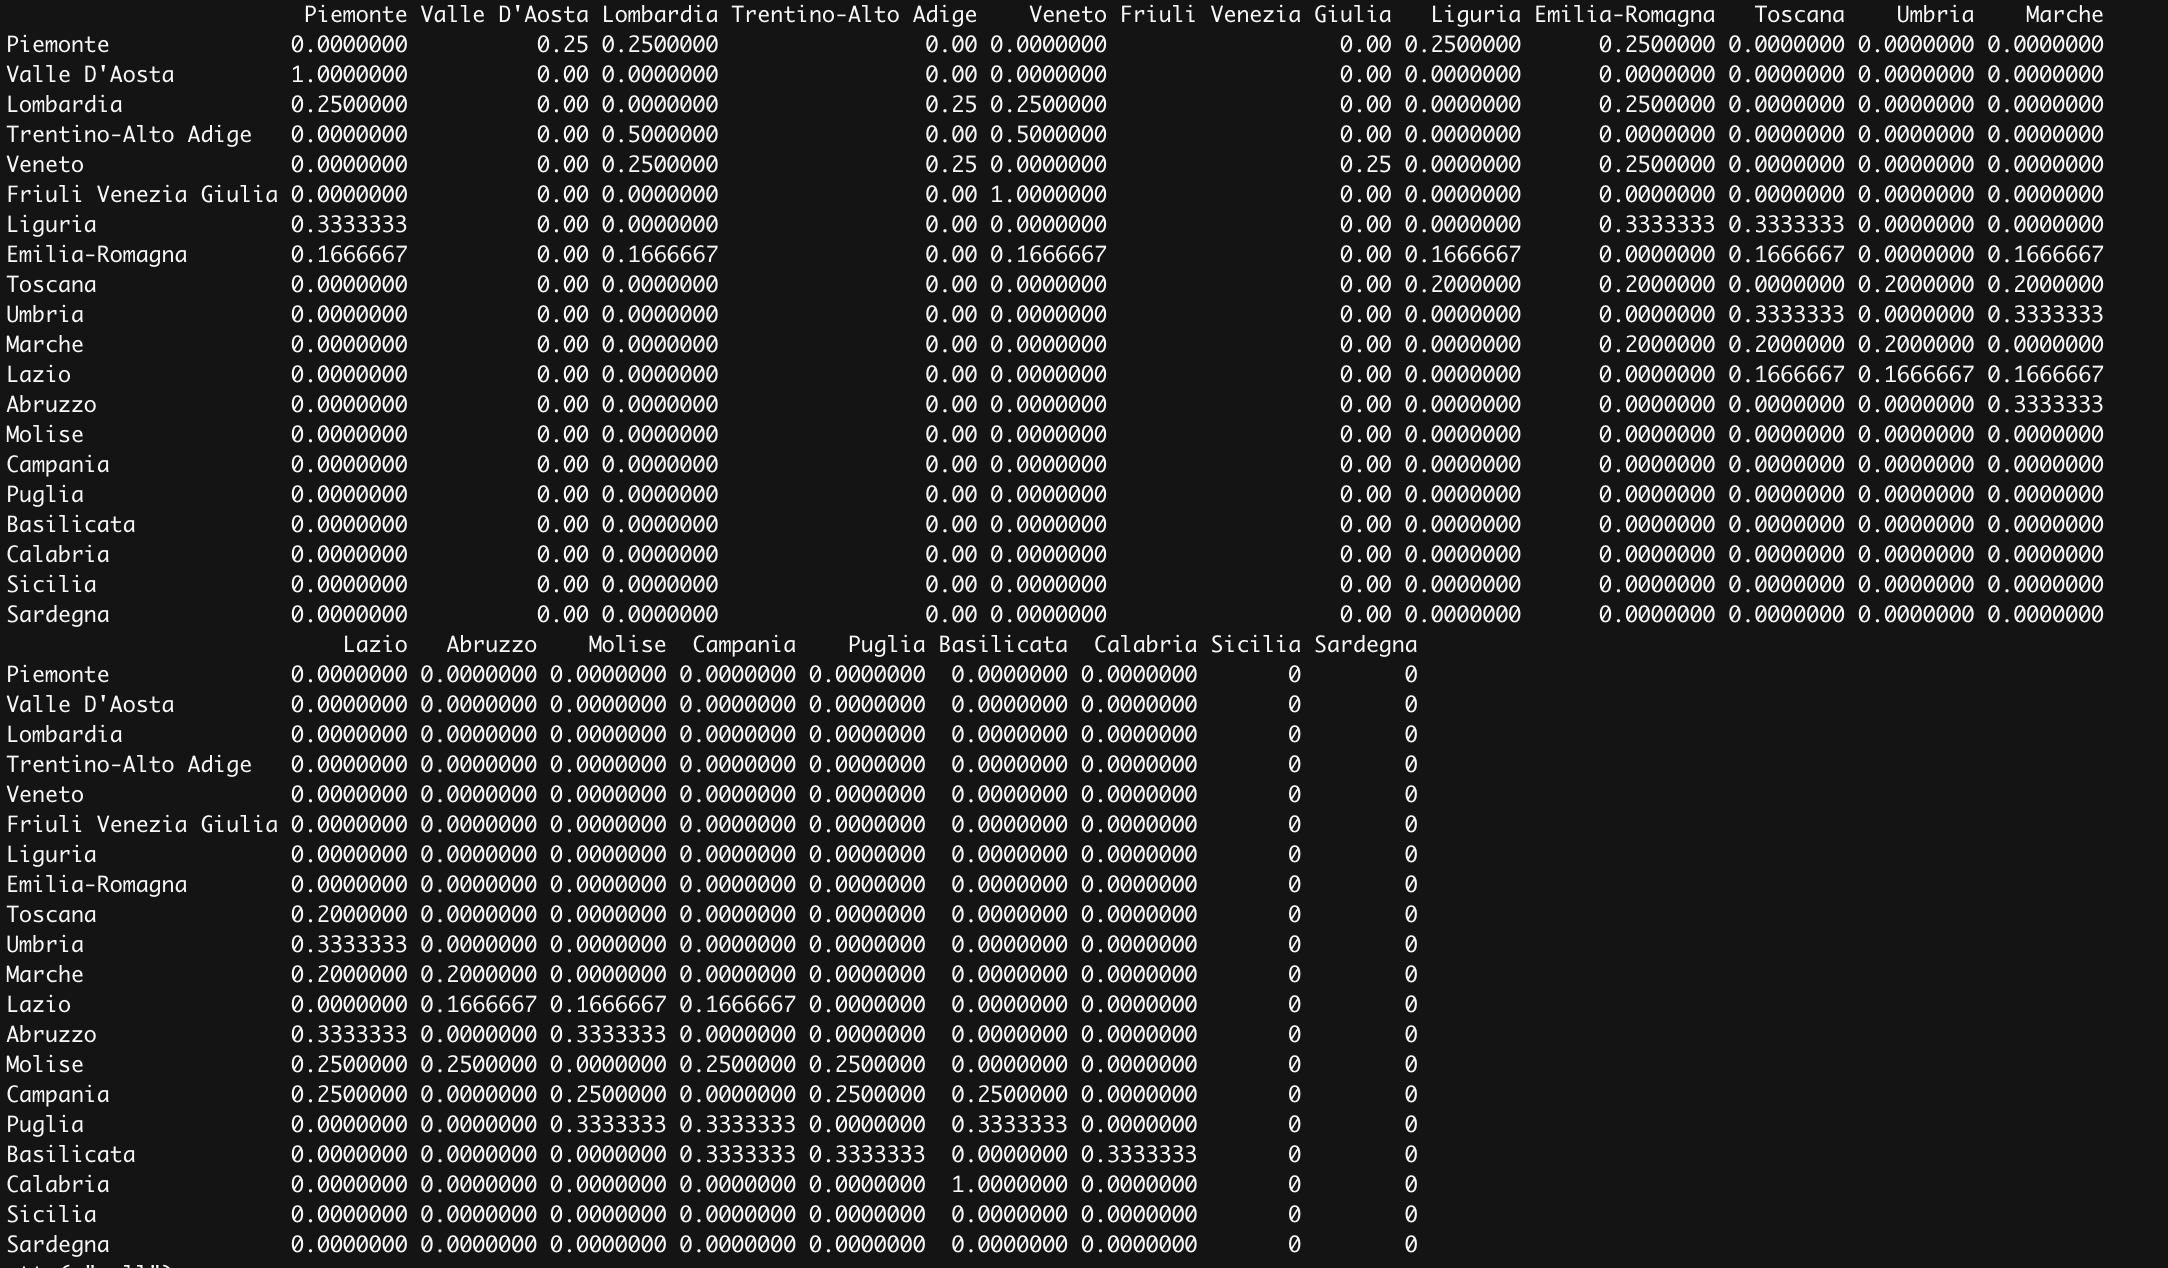
\includegraphics[scale=0.3]{figures/mat_italia}
   \end{figure}


\end{frame}

%----------------------------------------------------------------------%
\subsection{Weights Matrix in \texttt{R}}
%----------------------------------------------------------------------%
\begin{frame}[fragile]
\frametitle{Weights Matrix in \texttt{R}}


\begin{scriptsize}
\begin{Shaded}
\begin{Highlighting}[]
\KeywordTok{require}\NormalTok{(}\StringTok{"sf"}\NormalTok{)}
\KeywordTok{require}\NormalTok{(}\StringTok{"spdep"}\NormalTok{)}
\KeywordTok{require}\NormalTok{(}\StringTok{"dplyr"}\NormalTok{)}
\end{Highlighting}
\end{Shaded}

\begin{Shaded}
\begin{Highlighting}[]
\NormalTok{chi.poly\textless{}{-}}\KeywordTok{read\_sf}\NormalTok{(}\StringTok{"foreclosures/foreclosures.shp"}\NormalTok{)}
\KeywordTok{st\_crs}\NormalTok{(chi.poly) }\CommentTok{\#doesn't have a projection}
\end{Highlighting}
\end{Shaded}

\end{scriptsize}

\begin{verbatim}
## Coordinate Reference System: NA
\end{verbatim}

\begin{scriptsize}
\begin{Shaded}
\begin{Highlighting}[]
\KeywordTok{st\_crs}\NormalTok{(chi.poly)\textless{}{-}}\DecValTok{4326} \CommentTok{\#WGS84 set it in the map}
\end{Highlighting}
\end{Shaded}
\end{scriptsize}

\end{frame}

%----------------------------------------------------------------------%
\begin{frame}[fragile]
\frametitle{Weights Matrix in \texttt{R}}

\begin{scriptsize}

\begin{Shaded}
\begin{Highlighting}[]
\NormalTok{chi.poly\textless{}{-}}\KeywordTok{st\_transform}\NormalTok{(chi.poly,}\DecValTok{26916}\NormalTok{) }\CommentTok{\#reproject planarly}
\CommentTok{\#NAD83 UTM Zone 16N}
\KeywordTok{st\_crs}\NormalTok{(chi.poly)}
\end{Highlighting}
\end{Shaded}
\end{scriptsize}
\begin{tiny}
\begin{verbatim}
## Coordinate Reference System:
##   User input: EPSG:26916 
##   wkt:
## PROJCS["NAD83 / UTM zone 16N",
##     GEOGCS["NAD83",
##         DATUM["North_American_Datum_1983",
##             SPHEROID["GRS 1980",6378137,298.257222101,
##                 AUTHORITY["EPSG","7019"]],
##             TOWGS84[0,0,0,0,0,0,0],
##             AUTHORITY["EPSG","6269"]],
##         PRIMEM["Greenwich",0,
##             AUTHORITY["EPSG","8901"]],
##         UNIT["degree",0.0174532925199433,
##             AUTHORITY["EPSG","9122"]],
##         AUTHORITY["EPSG","4269"]],
##     PROJECTION["Transverse_Mercator"],
##     PARAMETER["latitude_of_origin",0],
##     PARAMETER["central_meridian",-87],
##     PARAMETER["scale_factor",0.9996],
##     PARAMETER["false_easting",500000],
##     PARAMETER["false_northing",0],
##     UNIT["metre",1,
##         AUTHORITY["EPSG","9001"]],
##     AXIS["Easting",EAST],
##     AXIS["Northing",NORTH],
##     AUTHORITY["EPSG","26916"]]
\end{verbatim}

\end{tiny}
\end{frame}

%----------------------------------------------------------------------%
\begin{frame}[fragile]
\frametitle{Weights Matrix in \texttt{R}}

\begin{scriptsize}
\begin{Shaded}
\begin{Highlighting}[]
\KeywordTok{str}\NormalTok{(chi.poly)}
\end{Highlighting}
\end{Shaded}
\end{scriptsize}
\begin{tiny}


\begin{verbatim}
## tibble [897 x 17] (S3: sf/tbl_df/tbl/data.frame)
##  $ SP_ID     : chr [1:897] "1" "2" "3" "4" ...
##  $ fips      : chr [1:897] "17031010100" "17031010200" "17031010300" "17031010400" ...
##  $ est_fcs   : int [1:897] 43 129 55 21 64 56 107 43 7 51 ...
##  $ est_mtgs  : int [1:897] 904 2122 1151 574 1427 1241 1959 830 208 928 ...
##  $ est_fcs_rt: num [1:897] 4.76 6.08 4.78 3.66 4.48 4.51 5.46 5.18 3.37 5.5 ...
##  $ res_addr  : int [1:897] 2530 3947 3204 2306 5485 2994 3701 1694 443 1552 ...
##  $ est_90d_va: num [1:897] 12.61 12.36 10.46 5.03 8.44 ...
##  $ bls_unemp : num [1:897] 8.16 8.16 8.16 8.16 8.16 8.16 8.16 8.16 8.16 8.16 ...
##  $ county    : chr [1:897] "Cook County" "Cook County" "Cook County" "Cook County" ...
##  $ fips_num  : num [1:897] 1.7e+10 1.7e+10 1.7e+10 1.7e+10 1.7e+10 ...
##  $ totpop    : int [1:897] 5391 10706 6649 5325 10944 7178 10799 5403 1089 3634 ...
##  $ tothu     : int [1:897] 2557 3981 3281 2464 5843 3136 3875 1768 453 1555 ...
##  $ huage     : int [1:897] 61 53 56 60 54 58 48 57 61 48 ...
##  $ oomedval  : int [1:897] 169900 147000 119800 151500 143600 145900 153400 170500 215900 114700 ...
##  $ property  : num [1:897] 646 914 478 509 641 612 678 332 147 351 ...
##  $ violent   : num [1:897] 433 421 235 159 240 266 272 146 78 84 ...
##  $ geometry  :sfc_POLYGON of length 897; first list element: List of 1
##   ..$ : num [1:15, 1:2] 443923 444329 444814 444839 444935 ...
##   ..- attr(*, "class")= chr [1:3] "XY" "POLYGON" "sfg"
##  - attr(*, "sf_column")= chr "geometry"
##  - attr(*, "agr")= Factor w/ 3 levels "constant","aggregate",..: NA NA NA NA NA NA NA NA NA NA ...
##   ..- attr(*, "names")= chr [1:16] "SP_ID" "fips" "est_fcs" "est_mtgs" ...
\end{verbatim}
\end{tiny}

\end{frame}


%----------------------------------------------------------------------%
\begin{frame}[fragile]
\frametitle{Weights Matrix in \texttt{R}}

\begin{scriptsize}
\begin{Shaded}
\begin{Highlighting}[]
\KeywordTok{plot}\NormalTok{(chi.poly[}\StringTok{\textquotesingle{}violent\textquotesingle{}}\NormalTok{])}
\end{Highlighting}
\end{Shaded}
\end{scriptsize}



  \begin{figure}[H] \centering
    \captionsetup{justification=centering}
    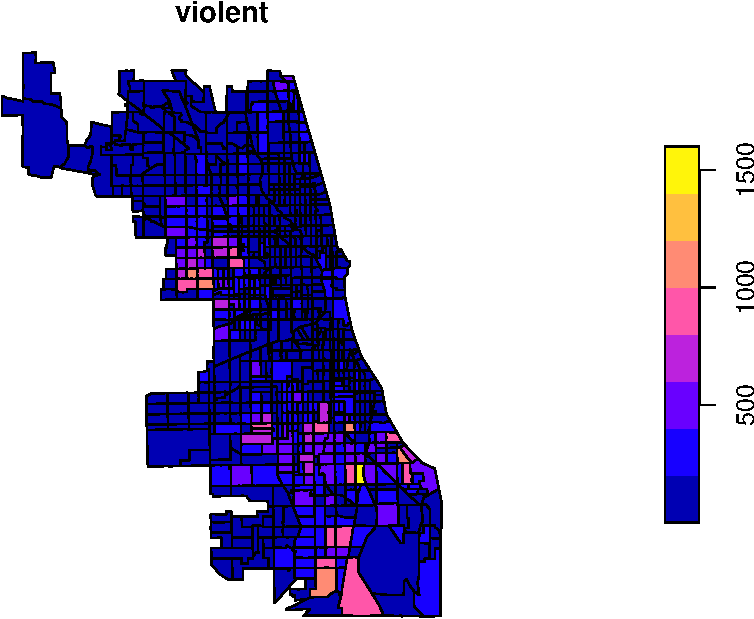
\includegraphics[scale=0.5]{Example_12_files/figure-latex/unnamed-chunk-2-1.pdf}
   \end{figure}



\end{frame}


%----------------------------------------------------------------------%
\begin{frame}[fragile]
\frametitle{Weights Matrix in \texttt{R}}


\begin{scriptsize}
\begin{Shaded}
\begin{Highlighting}[]
\NormalTok{list.queen\textless{}{-}}\KeywordTok{poly2nb}\NormalTok{(chi.poly, }\DataTypeTok{queen=}\OtherTok{TRUE}\NormalTok{)}
\NormalTok{W\textless{}{-}}\KeywordTok{nb2listw}\NormalTok{(list.queen, }\DataTypeTok{style=}\StringTok{"W"}\NormalTok{, }\DataTypeTok{zero.policy=}\OtherTok{TRUE}\NormalTok{)}
\NormalTok{W}
\end{Highlighting}
\end{Shaded}
\end{scriptsize}

\begin{tiny}
\begin{verbatim}
## Characteristics of weights list object:
## Neighbour list object:
## Number of regions: 897 
## Number of nonzero links: 6140 
## Percentage nonzero weights: 0.7631036 
## Average number of links: 6.845039 
## 
## Weights style: W 
## Weights constants summary:
##     n     nn  S0       S1       S2
## W 897 804609 897 274.4893 3640.864
\end{verbatim}

\end{tiny}

\end{frame}

%----------------------------------------------------------------------%
\begin{frame}[fragile]
\frametitle{Weights Matrix in \texttt{R}}


\begin{scriptsize}
\begin{Shaded}
\begin{Highlighting}[]
\KeywordTok{plot}\NormalTok{(W,}\KeywordTok{st\_geometry}\NormalTok{(}\KeywordTok{st\_centroid}\NormalTok{(chi.poly)))}
\end{Highlighting}
\end{Shaded}
\end{scriptsize}


 \begin{figure}[H] \centering
    \captionsetup{justification=centering}
    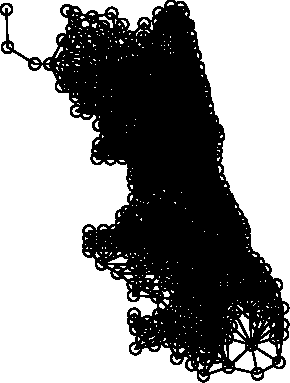
\includegraphics[scale=0.7]{Example_12_files/figure-latex/neighbors_plot-1.pdf}
   \end{figure}


\end{frame}

%----------------------------------------------------------------------%
\begin{frame}[fragile]
\frametitle{Weights Matrix in \texttt{R}}


\begin{scriptsize}
\begin{Shaded}
\begin{Highlighting}[]
\NormalTok{coords \textless{}{-}}\StringTok{ }\KeywordTok{st\_centroid}\NormalTok{(}\KeywordTok{st\_geometry}\NormalTok{(chi.poly), }\DataTypeTok{of\_largest\_polygon=}\OtherTok{TRUE}\NormalTok{)}
\NormalTok{W\_dist\textless{}{-}}\KeywordTok{dnearneigh}\NormalTok{(coords,}\DecValTok{0}\NormalTok{,}\DecValTok{1000}\NormalTok{)}
\NormalTok{W\_dist}
\end{Highlighting}
\end{Shaded}
\end{scriptsize}
\begin{tiny}
\begin{verbatim}
## Neighbour list object:
## Number of regions: 897 
## Number of nonzero links: 5448 
## Percentage nonzero weights: 0.6770991 
## Average number of links: 6.073579 
## 55 regions with no links:
## 141 142 143 145 153 154 155 158 462 631 637 638 642 643 644 645 655 656 657 658 659 758 759 769 820 821 822 823 824 855 856 857 861 862 864 865 866 867 868 870 871 872 873 876 877 880 885 886 887 888 889 890 892 896 897
\end{verbatim}

\end{tiny}


\begin{scriptsize}
\begin{Shaded}
\begin{Highlighting}[]
\KeywordTok{plot}\NormalTok{(W\_dist, coords)}
\end{Highlighting}
\end{Shaded}

\end{scriptsize}


 \begin{figure}[H] \centering
    \captionsetup{justification=centering}
    
\includegraphics[scale=0.7]{Example_12_files/figure-latex/unnamed-chunk-3-1.pdf}
   \end{figure}



\end{frame}

%----------------------------------------------------------------------%
\begin{frame}[fragile]
\frametitle{Weights Matrix in \texttt{R}}

\begin{scriptsize}
\begin{Shaded}
\begin{Highlighting}[]
\NormalTok{W\_dist\textless{}{-}}\KeywordTok{dnearneigh}\NormalTok{(coords,}\DecValTok{0}\NormalTok{,}\DecValTok{4300}\NormalTok{)}
\NormalTok{W\_dist}
\end{Highlighting}
\end{Shaded}
\end{scriptsize}

\begin{tiny}
\begin{verbatim}
## Neighbour list object:
## Number of regions: 897 
## Number of nonzero links: 87988 
## Percentage nonzero weights: 10.9355 
## Average number of links: 98.09142
\end{verbatim}
\end{tiny}

\begin{scriptsize}
\begin{Shaded}
\begin{Highlighting}[]
\KeywordTok{plot}\NormalTok{(W\_dist, coords)}
\end{Highlighting}
\end{Shaded}
\end{scriptsize}


 \begin{figure}[H] \centering
    \captionsetup{justification=centering}
    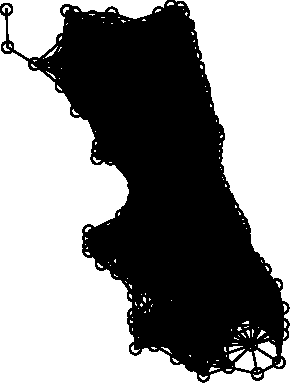
\includegraphics[scale=0.7]{Example_12_files/figure-latex/unnamed-chunk-4-1.pdf}
   \end{figure}



\end{frame}


%----------------------------------------------------------------------%
\section{Traditional Spatial Regressions }
%----------------------------------------------------------------------%
\begin{frame}[fragile]
\frametitle{Traditional Spatial Econometrics }
\framesubtitle{Spatial Autoregressive (SAR) Models}

\begin{itemize}
\item Spatial lag dependence in a regression setting can be modeled similar to
an autoregressive process in time series. Formally,
\end{itemize}


\[ y= \rho Wy+ X \beta + \epsilon \]

\begin{itemize}
  \footnotesize
\item \(Wy\) induces a nonzero correlation with the error term, similar to the presence of an endogenous variable.

\item  Unlike to time series, \(Wy_i\) is always correlated with \(\epsilon_i\) 

\item OLS estimates in the non spatial model will be biased and inconsistent. (Anselin and Bera, 1998)

\item The estimation of the SAR model can be approached in two ways.
\begin{enumerate}
  \tiny
  \item Assume normality of the error term and use maximum likelihood.
  \item Use 2SLS
\end{enumerate}
\item In \texttt{R}  the function \texttt{lagsarlm} uses MLE
\end{itemize}

\end{frame}

%----------------------------------------------------------------------%
\section{Prediction with SAR Models}
%----------------------------------------------------------------------%
\begin{frame}[fragile]
\frametitle{Prediction with SAR Models}

\begin{itemize}
  \item The usual {\it prolegomena}
\end{itemize}


\begin{scriptsize}
\begin{Shaded}
\begin{Highlighting}[]
\KeywordTok{set.seed}\NormalTok{(}\DecValTok{101010}\NormalTok{) }\CommentTok{\#sets a seed }
\CommentTok{\#70\% train}
\NormalTok{indic\textless{}{-}}\KeywordTok{sample}\NormalTok{(}\DecValTok{1}\OperatorTok{:}\KeywordTok{nrow}\NormalTok{(chi.poly),}\KeywordTok{floor}\NormalTok{(.}\DecValTok{7}\OperatorTok{*}\KeywordTok{nrow}\NormalTok{(chi.poly)))}

\CommentTok{\#Partition the sample}
\NormalTok{train\textless{}{-}chi.poly[indic,]}
\NormalTok{test\textless{}{-}chi.poly[}\OperatorTok{{-}}\NormalTok{indic,]}


\NormalTok{ols\textless{}{-}}\KeywordTok{lm}\NormalTok{(violent}\OperatorTok{\textasciitilde{}}\NormalTok{est\_fcs\_rt}\OperatorTok{+}\NormalTok{bls\_unemp, }\DataTypeTok{data=}\NormalTok{train)}
\NormalTok{test}\OperatorTok{$}\NormalTok{yhat\textless{}{-}}\KeywordTok{predict}\NormalTok{(ols,}\DataTypeTok{newdata=}\NormalTok{test)}
\KeywordTok{mean}\NormalTok{((test}\OperatorTok{$}\NormalTok{violent}\OperatorTok{{-}}\NormalTok{test}\OperatorTok{$}\NormalTok{yhat)}\OperatorTok{\^{}}\DecValTok{2}\NormalTok{)}
\end{Highlighting}
\end{Shaded}

\begin{verbatim}
## [1] 29773.64
\end{verbatim}
\end{scriptsize}
\end{frame}

%----------------------------------------------------------------------%
\begin{frame}[fragile]
\frametitle{Prediction with SAR Models}

\begin{itemize}
  \item Modeling the spatial structure with a SAR Model
\end{itemize}


\begin{scriptsize}
\begin{Shaded}
\begin{Highlighting}[]
\NormalTok{list.queen\_train\textless{}{-}}\KeywordTok{poly2nb}\NormalTok{(train, }\DataTypeTok{queen=}\OtherTok{TRUE}\NormalTok{)}
\NormalTok{W\_train\textless{}{-}}\KeywordTok{nb2listw}\NormalTok{(list.queen\_train, }\DataTypeTok{style=}\StringTok{"W"}\NormalTok{, }\DataTypeTok{zero.policy=}\OtherTok{TRUE}\NormalTok{)}
\NormalTok{W\_train}

\ErrorTok{Error in print.listw(x) : regions with no neighbours found, use zero.policy=TRUE}

\KeywordTok{plot}\NormalTok{(train[}\StringTok{"fips"}\NormalTok{])}
\end{Highlighting}
\end{Shaded}
\end{scriptsize}

\begin{figure}[H] \centering
    \captionsetup{justification=centering}
    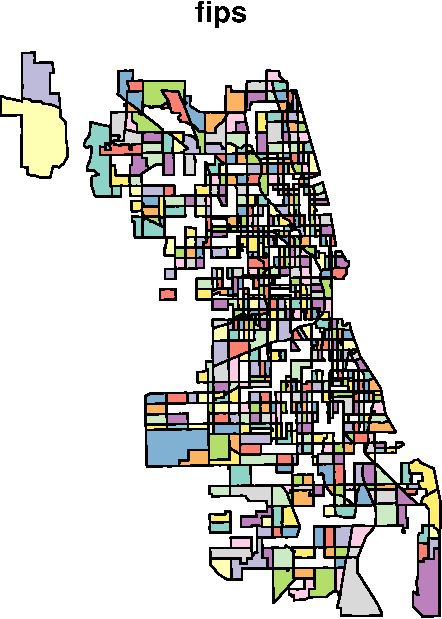
\includegraphics[scale=0.4]{Example_12_files/figure-latex/unnamed-chunk-8-1.pdf}
   \end{figure}


\end{frame}

%----------------------------------------------------------------------%
\begin{frame}[fragile]
\frametitle{Prediction with SAR Models}

\begin{itemize}
  \item Use distance instead
\end{itemize}

\begin{scriptsize}


\begin{Shaded}
\begin{Highlighting}[]

\NormalTok{coords \textless{}{-}}\StringTok{ }\KeywordTok{st\_centroid}\NormalTok{(}\KeywordTok{st\_geometry}\NormalTok{(train), }\DataTypeTok{of\_largest\_polygon=}\OtherTok{TRUE}\NormalTok{)}
\NormalTok{W\_train\textless{}{-}}\KeywordTok{dnearneigh}\NormalTok{(coords,}\DecValTok{0}\NormalTok{,}\DecValTok{4300}\NormalTok{)}
\NormalTok{W\_train\textless{}{-}}\KeywordTok{nb2listw}\NormalTok{(W\_train, }\DataTypeTok{style=}\StringTok{"W"}\NormalTok{, }\DataTypeTok{zero.policy=}\OtherTok{TRUE}\NormalTok{)}



\NormalTok{coords \textless{}{-}}\StringTok{ }\KeywordTok{st\_centroid}\NormalTok{(}\KeywordTok{st\_geometry}\NormalTok{(test), }\DataTypeTok{of\_largest\_polygon=}\OtherTok{TRUE}\NormalTok{)}
\NormalTok{W\_test\textless{}{-}}\KeywordTok{dnearneigh}\NormalTok{(coords,}\DecValTok{0}\NormalTok{,}\DecValTok{4300}\NormalTok{)}
\NormalTok{W\_test\textless{}{-}}\KeywordTok{nb2listw}\NormalTok{(W\_test, }\DataTypeTok{style=}\StringTok{"W"}\NormalTok{, }\DataTypeTok{zero.policy=}\OtherTok{TRUE}\NormalTok{)}



\KeywordTok{require}\NormalTok{(}\StringTok{"spatialreg"}\NormalTok{)}

\NormalTok{sar.chi\textless{}{-}}\KeywordTok{lagsarlm}\NormalTok{(violent}\OperatorTok{\textasciitilde{}}\NormalTok{est\_fcs\_rt}\OperatorTok{+}\NormalTok{bls\_unemp, }\DataTypeTok{data=}\NormalTok{train, W\_train)}

\NormalTok{test}\OperatorTok{$}\NormalTok{yhat\_sar\textless{}{-}}\KeywordTok{predict}\NormalTok{(sar.chi,}\DataTypeTok{newdata=}\NormalTok{test,}\DataTypeTok{listw=}\NormalTok{W\_test)}
\end{Highlighting}
\end{Shaded}

\end{scriptsize}

\end{frame}

%----------------------------------------------------------------------%
\begin{frame}[fragile]
\frametitle{Prediction with SAR Models}

\begin{itemize}
  \item Comparing to OLS
\end{itemize}

\begin{Shaded}
\begin{Highlighting}[]
\KeywordTok{mean}\NormalTok{((test}\OperatorTok{$}\NormalTok{violent}\OperatorTok{{-}}\NormalTok{test}\OperatorTok{$}\NormalTok{yhat)}\OperatorTok{\^{}}\DecValTok{2}\NormalTok{)}
\end{Highlighting}
\end{Shaded}

\begin{verbatim}
## [1] 29773.64
\end{verbatim}

\begin{Shaded}
\begin{Highlighting}[]
\KeywordTok{mean}\NormalTok{((test}\OperatorTok{$}\NormalTok{violent}\OperatorTok{{-}}\NormalTok{test}\OperatorTok{$}\NormalTok{yhat\_sar)}\OperatorTok{\^{}}\DecValTok{2}\NormalTok{)}
\end{Highlighting}
\end{Shaded}

\begin{verbatim}
## [1] 28662.23
\end{verbatim}

\end{frame}
%----------------------------------------------------------------------%
\begin{frame}

\frametitle{Review \& Next Steps}
  
  \begin{itemize} 
    \item Today:
    \medskip
    \begin{itemize} 
        \item Closeness
        \medskip
        \item Weights Matrix
        \medskip
        \item Examples of Weight Matrices Weights Matrix in R
        \medskip
        \item Traditional Spatial Regressions
        \medskip
        \item Prediction with SAR Models
      \end{itemize}
  	\bigskip  

	\item  Next class: More on Spatial Regressions


\bigskip  
\item Questions? Questions about software? 

\end{itemize}
\end{frame}

%----------------------------------------------------------------------%
\section{Further Readings}
%----------------------------------------------------------------------%
\begin{frame}
\frametitle{Further Readings}

\begin{itemize}

   
  \item Arbia, G. (2014). A primer for spatial econometrics with applications in R. Palgrave Macmillan. (Chapter 2 and 3)
  \medskip
  \item Anselin, Luc, \& Anil K Bera. 1998. “Spatial Dependence in Linear Regression Models with an Introduction to Spatial Econometrics.” Statistics Textbooks and Monographs 155. MARCEL DEKKER AG: 237–90.
  \medskip
  \item Sarmiento-Barbieri, I. (2016). An Introduction to Spatial Econometrics in R. \url{http://www.econ.uiuc.edu/~lab/workshop/Spatial_in_R.html}
  \medskip
  \item Tobler, WR. 1979. “Cellular Geography.” In Philosophy in Geography, 379–86. Springer.
\end{itemize}

\end{frame}






%----------------------------------------------------------------------%
%----------------------------------------------------------------------%
\end{document}
%----------------------------------------------------------------------%
%----------------------------------------------------------------------%

